%% Diagram to illustrate the algorithm
\documentclass[8pt, tikz]{standalone}

\usepackage{times}

\usetikzlibrary{arrows.meta, bending, decorations.pathreplacing, positioning, shapes}

\begin{document}
  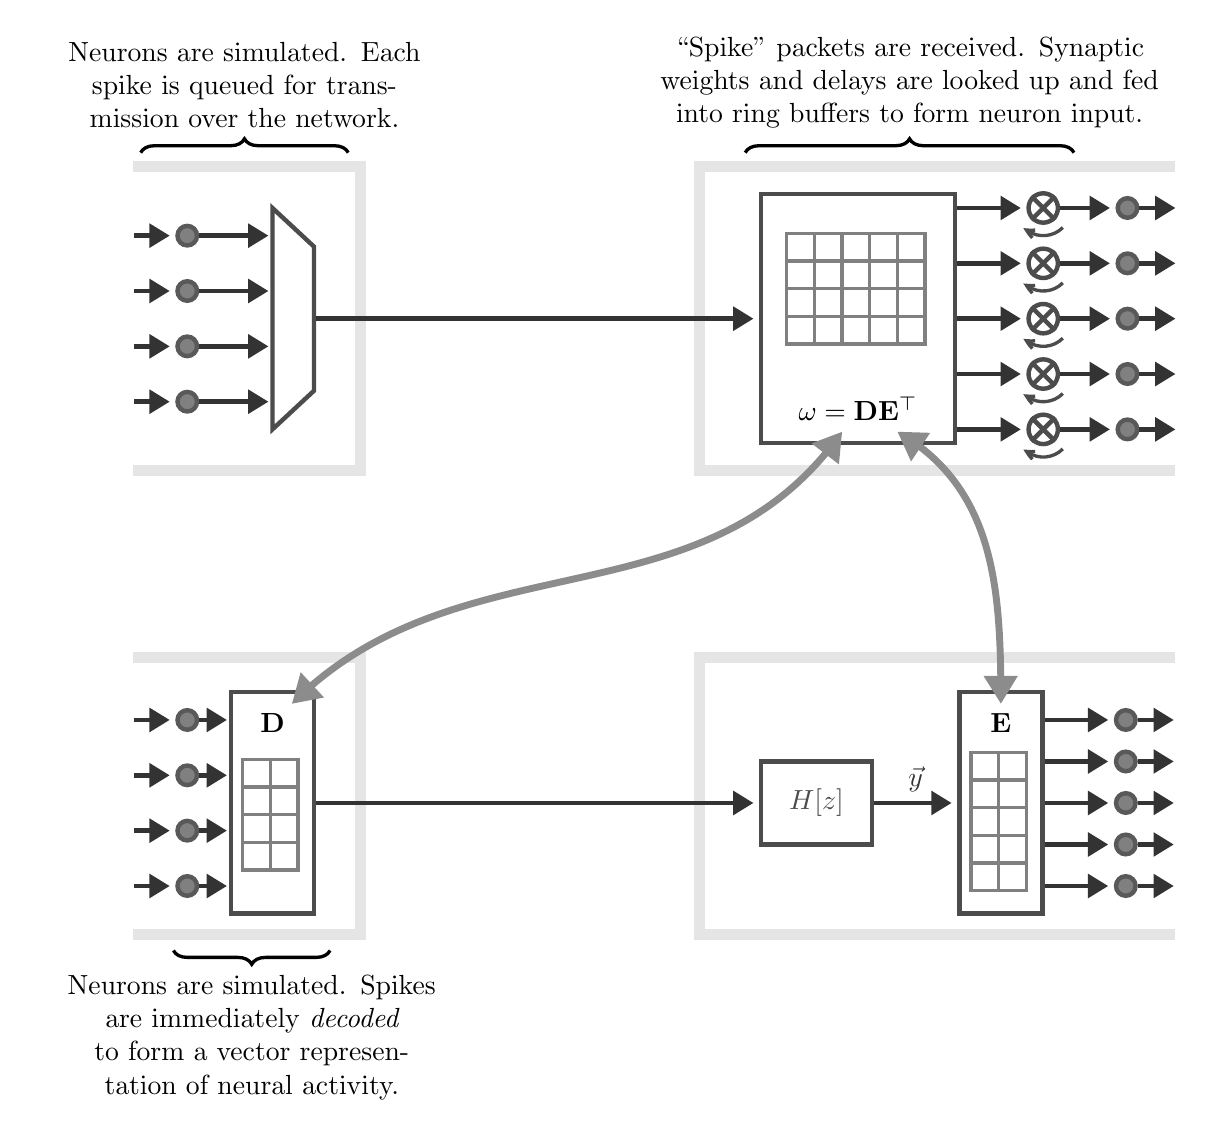
\begin{tikzpicture}[
    neuron/.style = {
      fill=gray, circle, text width=5pt, text height=5pt, inner sep=0,
      draw=black!65!white, ultra thick,
    },
    box/.style = {
      ultra thick, color=black!70!white, draw,
    },
    ringbuffer/.style = {
      box, circle, text width=7.5pt, text height=7.5pt, inner sep=0,
    },
    matrix line/.style = {very thick, draw=black!50!white},
    relation/.style = {line width=2.5pt, black!45!white, arrows={Triangle[]-Triangle[]}},
    core/.style = {line width=4pt, line cap=rect, black!10!white},
    link/.style = {ultra thick, black!80!white, arrows={-Triangle[]}, shorten >= 2pt},
    brace/.style = {decoration={brace, amplitude=5pt}, decorate, very thick},
    brace label/.style = {midway, align=center},
    brace label above/.style = {brace label, above=5pt},
    brace label below/.style = {brace label, below=5pt},
  ]
    %% Draw the spike-transmission algorithm
    \begin{scope}
      %% Draw the processing cores
      \draw [core]
        (-17.5pt, -25pt) -| ++(80pt, 110pt) -- ++(-80pt, 0);
      \draw [core]
        (355pt, 85pt) -| ++(-170pt, -110pt) -- ++(170pt, 0);

      %% Draw the neurons in the first processing core
      \foreach \n in {0,...,3}{%
        \node [neuron] (spike1\n) at (0, \n*20pt) {};
        \draw [link] ([xshift=-15pt] spike1\n.west) -- (spike1\n.west);
      }

      %% The multiplex which takes spikes and produces packets.
      \node [trapezium, box, rotate=-90,
             minimum width=80pt, minimum height=15pt,
             anchor=south, trapezium stretches, trapezium angle=75]
        (spike-mux) at (30pt, 30pt) {};

      %% Communication of spikes to the mux
      \foreach \n in {0,...,3}{%
        \draw [link] (spike1\n.east) -- ++(27pt, 0);
      }

      %% The synaptic weight lookup table in the next processing core
      \node [box, minimum width=70pt, minimum height=90pt,
             right=160pt of spike-mux.north]
        (spike-lut) {};

      %% Draw the synaptic weight matrix inside the memory
      \begin{scope}[matrix line]
        \draw ([xshift=10pt, yshift=-15pt] spike-lut.north west) rectangle ++(50pt, -40pt);
        \foreach \n in {1,...,4}{%
          \draw ([xshift=10pt + \n*10pt, yshift=-15pt] spike-lut.north west)
                -- ++(0pt, -40pt);
        }
        \foreach \n in {1,...,3}{%
          \draw ([xshift=10pt, yshift=-15pt - \n*10pt] spike-lut.north west)
                -- ++(50pt, 0pt);
        }
        \node [above=5pt of spike-lut.south] (label-wm) {$\omega = \mathbf{D}\mathbf{E}^\top$};
      \end{scope}

      %% Draw the packet stream from mux to LUT
      \draw [link] (spike-mux) -- (spike-lut);

      %% Draw the ring buffers and neurons
      \foreach \n in {0,...,4}{%
        \node [right=25pt of spike-lut, ringbuffer,
               yshift=\n*20pt - 40pt] (spike-rb\n) {};
        \draw [box, very thick, arrows={-Straight Barb[bend, width=3pt, length=3pt]}]
          (spike-rb\n.center)++(-45:10pt)
          arc [start angle=-45, delta angle=-90, x radius=10pt, y radius=10pt];
        \draw [link] ([yshift=\n*20pt - 40pt] spike-lut.east) -- (spike-rb\n);
        \draw [box] (spike-rb\n.north west) -- (spike-rb\n.south east);
        \draw [box] (spike-rb\n.south west) -- (spike-rb\n.north east);


        \node [right=20pt of spike-rb\n, neuron] (spike2\n) {};
        \draw [link] (spike-rb\n) -- (spike2\n);
        \draw [link] (spike2\n.east) -- ++(15pt, 0);
      }
    \end{scope}

    %% Draw the value-transmission algorithm
    \begin{scope}[yshift=-175pt]
      %% Draw the processing cores
      \draw [core]
        (-17.5pt, -17.5pt) -| ++(80pt, 100pt) -- ++(-80pt, 0);
      \draw [core]
        (355pt, 82.5pt) -| ++(-170pt, -100pt) -- ++(170pt, 0);

      %% Draw the neurons in the first processing core
      \foreach \n in {0,...,3}{%
        \node [neuron] (value1\n) at (0, \n*20pt) {};
        \draw [link] ([xshift=-15pt] value1\n.west) -- (value1\n.west);
      }

      %% The decoder which takes spikes and results in value packets
      \node [box, anchor=west, minimum height=80pt, minimum width=30pt]
        (value-decoder) at (15pt, 30pt) {};
      \begin{scope}[matrix line]
        \draw ([xshift=5pt, yshift=-25pt] value-decoder.north west) rectangle ++(20pt, -40pt);
        \draw ([xshift=15pt, yshift=-25pt] value-decoder.north west) -- ++(0, -40pt);
        \foreach \n in {1,...,3}{%
          \draw ([xshift=5pt, yshift=-25pt - 10pt*\n] value-decoder.north west) -- ++(20pt, 0);
        }
      \end{scope}
      \node [below=5pt of value-decoder.north] (label-d) {$\mathbf{D}$};

      %% Communication of spikes to the decoder
      \foreach \n in {0,...,3}{%
        \draw [link] (value1\n.east) -- ++(12pt, 0);
      }

      %% The synaptic filter and encoder in the next core
      \node [box, minimum width=40pt, minimum height=30pt,
             right=160pt of value-decoder.east]
           (value-filter) {$H[z]$};
      \node [box, minimum height=80pt, minimum width=30pt,
             right=30pt of value-filter.east]
        (value-encoder) {};
      \begin{scope}[matrix line]
        \draw ([xshift=5pt, yshift=-22.5pt] value-encoder.north west)
          rectangle ++(20pt, -50pt);
        \draw ([xshift=15pt, yshift=-22.5pt] value-encoder.north west)
          -- ++(0, -50pt);
        \foreach \n in {1,...,4}{%
          \draw ([xshift=5pt, yshift=-22.5pt - 10pt*\n] value-encoder.north west)
            -- ++(20pt, 0);
        }
      \end{scope}
      \node [below=5pt of value-encoder.north] (label-e) {$\mathbf{E}$};

      %% Draw the packet stream across the network
      \draw [link] (value-decoder) -- (value-filter);

      %% Draw the packet stream from filter to encoder
        \draw [link] (value-filter) -- (value-encoder) node [midway, above] {$\vec{y}$};

      %% Draw the neurons
      \foreach \n in {0,...,4}{%
        \node [right=25pt of value-encoder, yshift=\n*15pt - 30pt, neuron] (value2\n) {};
        \draw [link] ([yshift=\n*15pt - 30pt] value-encoder.east) -- (value2\n);
        \draw [link] (value2\n.east) -- ++(15pt, 0);
      }
    \end{scope}

    %% Connect up relevant components between the two
    \draw [relation] (label-d) to [out=45, in=235] (label-wm);
    \draw [relation] (label-e) to [out=90, in=-30] (label-wm);

    %% Label the diagram
    %% Label the spike based system
    %% Neurons
    \draw [brace] ([xshift=-12.5pt, yshift=30pt] spike13.west) -- ++(75pt, 0pt)
      node [brace label above, text width=150pt] {
        Neurons are simulated.
        Each spike is queued for transmission over the network.
      }
      node [pos=1, coordinate] (topbrace) {};

    %% Receiving and synaptic weights
      \draw [brace]
        ([xshift=-5pt] spike-lut.north west |- topbrace) --
        ([xshift=5pt] spike-rb3.east |- topbrace)
        node [brace label above, text width=200pt] {``Spike'' packets are received.  Synaptic weights and delays are looked up and fed into ring buffers to form neuron input.};


    %% Label the value based system
    \draw [brace] ([xshift=5pt, yshift=-12.5pt] value-decoder.south east) --
                  ([xshift=-5pt, yshift=-12.5pt] value10 |- value-decoder.south east)
                  node [brace label below, text width=150pt] {Neurons are simulated.  Spikes are immediately \textit{decoded} to form a vector representation of neural activity.}
      node [pos=1] (botbrace) {};
  \end{tikzpicture}
\end{document}
